\chapter{Integración de los ejercicios en Robotics Academy}
\label{cap:capitulo5}

En este capítulo profundizaremos en el proceso creativo de la infraestructura de los dos ejercicios Follow Person para Robotics Academy para dar al usuario una plantilla web óptima con el que pueda desarrollar el algoritmo cómodamente.\\




% -- SECCION ENTORNO GAZEBO
% ---------------------------
\section{Entorno simulado de un hospital}
\label{sec:hospital_gazebo}

La primera tarea fue integrar un escenario de Gazebo para el ejercicio \textit{Follow Person} simulado. El escenario candidato que elegimos fue un Hospital debido a las siguientes ventajas:

\begin{enumerate}
	\item El robot se enfrenta a un \textit{entorno} complejo (paredes, obstáculos, varias personas).
	\item La tarea Sigue Personas tiene lugar en un entorno en el cuál tiene sentido verlo en el mundo real. Los Robots en el ámbito de la salud están en continua integración y más desde el año 2020.
\end{enumerate}

De modo que incorporamos el siguiente escenario de Gazebo que proporciona AWS (Amazon Web Service) en uno de sus repositorios de Github \footnote{\textbf{aws hospital}: \url{https://github.com/aws-robotics/aws-robomaker-hospital-world}}:\\

\begin{figure} [H]
  \begin{center}
    \includegraphics[width=10cm]{imagenes/cap5/hospital_world.png}
  \end{center}
  \caption[Hospital de AWS en Gazebo]{Hospital de AWS en Gazebo}
  \label{fig:hospital_gazebo}
\end{figure}\

El repositorio proporcionaba varios ficheros \textit{.world} con distintas versiones del Hospital: solo planta baja, una planta y dos plantas. Elegimos por comodidad la primera.\\

El siguiente paso era integrar una persona que pudiera desplazarse por el entorno.\\



% -- SECCION TELEOPERADOR
% -------------------------
\section{Teleoperador}
\label{sec:teleoperador}

La meta final es que el usuario que use la plantilla web pueda controlar manualmente una persona del Hospital para que el robot pueda seguirla. Para ello teníamos que desarrollar un \textit{teleoperador}.\\

El primer punto de partida era integrar una persona en el nuevo entorno simulado, por lo que accedimos a este repositorio: \url{https://github.com/osrf/gazebo_models} que incorpora una librería de modelos para Gazebo e incorporamos el modelo \textit{person standing} en el repositorio de Robotics Academy de terceros \textit{Custom Robots}\\

\begin{figure} [H]
  \begin{center}
    \includegraphics[width=10cm]{imagenes/cap5/person_model.png}
  \end{center}
  \caption[Persona simulada en Gazebo]{Persona simulada en Gazebo}
  \label{fig:persona_gazebo}
\end{figure}\

Ahora bien, el modelo es \textit{estático}, carece de capacidad de desplazamiento, por lo que fue necesario desarrollar un \textit{plugin} para Gazebo que permitiera controlarlo o que pudiera desplazarse a través de una ruta que eligiera el programador. De modo que en el mismo paquete donde teníamos los ficheros de lanzamiento del hospital diseñamos el \textit{plugin} (escrito en C++) que denominamos \textit{libpersonplugin.so} para incorporarlo en el fichero \textit{.sdf} (similar a URDF) de la persona. En este enlace podréis ver el \textbf{código fuente}\footnote{\textbf{person plugin}: \url{https://github.com/JdeRobot/CustomRobots/blob/foxy-devel/amazon_hospital/hospital_world/src/person.cpp}}. Como punto de partida, tomamos como referencia un \textit{plugin} de una persona simulada que hizó \textit{Pedro Arias} en su TFM\footnote{\textbf{TFM Pedro Arias}: \url{https://github.com/RoboticsLabURJC/2021-tfm-pedro-arias}}\\

El plugin requiere 2 funcionalidades:
\begin{enumerate}
	\item Comunicación remota para el control manual. La intención es que el usuario se comunique con el modelo simulado, por lo tanto, se ha diseñado un \textit{socket} de comunicaciones para dicha tarea.
	\item Establecimiento de una ruta por defecto y capacidad de incorporar nuevas rutas. Esta última funcionalidad no es necesaria para el ejercicio, además de que puede suponer cierta molestia al usuario, pero no se descarta su utilidad para un futuro. Básicamente, dado un vector de tuplas de tipo $<$float, float, int$>$ donde los 2 primeros elementos indican la posición X e Y y el último parámetro apuntando al siguiente punto de paso, podemos implementar una ruta en un bucle infinito (el último punto de paso tiene que apuntar al primero).
\end{enumerate}\




% -- SUBSECCION COMUNICACION REMOTA
% ----------------------------------
\subsection{Comunicación remota}
\label{subsec:comunicacion_remota}

En el propio fichero \textit{person.cpp} se crearon 2 hilos (threads): uno actuaría como servidor de un socket de comunicaciones que usaría el protocolo de transporte UDP (No esta orientado a la conexión y es más rápido) y otro hilo se encargaría de actualizar la posición del modelo. Dentro del socket se implementó un protocolo de comunicación que entendierá el servidor, el cual se comportara únicamente como receptor de los mensajes del cliente. Los mensajes (de 3 caracteres) que puede recibir son:\\

\begin{itemize}
	\item \textbf{``UVF"} (User Velocity Forward). El modelo se mueve hacia delante.
	\item \textbf{``UVB"} (User Velocity Backward). El modelo se mueva hacia atrás.
	\item \textbf{``UAR"} (User Angular Right). El modelo gira hacia la derecha.
	\item \textbf{``UAL"} (User Angular Left). El modelo gira hacia la izquiera.
	\item \textbf{``US-"} (User Stop). El modelo se detiene.
	\item \textbf{``A--"} (Autonomous). El modelo pasa a modo autónomo. Sigue la ruta establecida (actualmente desactivada).
\end{itemize}\

Pero ¿dónde entra en juego el cliente? El fichero \textit{exercise.py} incorpora un socket de comunicación UDP que se conecta al servidor del \textit{plugin} a través del puerto 36677. Además, el exercise.py actúa como servidor de un WebSocket en comunicación con la plantilla web. Cuando el usuario haga click en el botón ``Teleoperate", el fichero de eventos de JavaScript enviará a través de un Websocket (usa el puerto 1905) las teclas pulsadas para que el exercise.py se lo retransmita al \textit{plugin}. Al iguál que en la comunicación plugin-exercise.py, se implementó un protocolo de comunicación para exercise.py-exercise.html. Los mensajes que puede recibir son:\\

\begin{itemize}
	\item \textbf{``\#teleop\_true"}. Activa la teleoperación. A partir de ese momento, el usuario puede pulsar los botones ``awsdx". Envía un mensaje \textbf{``US-"} al plugin.
	\item \textbf{``\#teleop\_false"}. Desactiva la teleoperación. Pasa a modo autónomo (si estuviera activado). Envía una mensaje \textbf{``A--"} al plugin.
	\item \textbf{``\#key\_a"}. Envía un mensaje \textbf{``UAR"} al plugin.
	\item \textbf{``\#key\_d"}. Envía un mensaje \textbf{``UAL"} al plugin.
	\item \textbf{``\#key\_w"}. Envía un mensaje \textbf{``UVF"} al plugin.
	\item \textbf{``\#key\_s"}. Envía un mensaje \textbf{``UVB"} al plugin.
	\item \textbf{``\#key\_x"}. Envía un mensaje \textbf{``US-"} al plugin.
\end{itemize}\

A continuación podemos ver un esquema que resuma la comunicación existente entre el exercise.html (incorpora el fichero ws\_code.js que es el manejador de eventos del menú superior de la plantilla web) con el plugin:\\

\begin{figure} [H]
  \begin{center}
    \includegraphics[width=15cm]{imagenes/cap5/comunicacion-teleoperador.png}
  \end{center}
  \caption[Comunicación del teleoperador]{Comunicación del teleoperador}
  \label{fig:comunicacion_teleoperador}
\end{figure}\

\cleardoublepage




% -- SECCION RNA
% ----------------
\section{Elección de RNA para detección de Objetos}
\label{sec:eleccion_rna}

La elección de una RNA que pueda detectar objetos se basó en este criterio: tiene que ejecutar de manera óptima en una CPU o en un contenedor Docker sin aceleración gráfica para permitir al usuario la ópción de programar cómodamente y poder disfrutar igualmente de la experiencia. Para ello, hicimos un previo estudio de los FPS (fotogramas por segundo) cuando se usan estos 2 modelos de RNA en una aplicación de Visión Artificial: YOLO a través de Darknet ROS y SSD Inceptión V2 (ambos mencionados en el capítulo 1 como arquitecturas de redes convolucionales [\ref{subsec:redes_convolucionales}]).\\

Primero probamos un paquete \textit{fork}\footnote{\textbf{Darknet ROS}: \url{https://github.com/Ar-Ray-code/darknet_ros/tree/foxy/darknet_ros/}} del repositorio oficial de \textit{Darknet ROS} para ROS2 Foxy que incluía un fichero de lanzamiento \textit{yolov4-tiny.launch.py} que ejecutaba una RNA profunda con menos capas que la original, provocando un aumento de rendimiento pero menor precisión. La ventaja de usar Darknet ROS es que indicas en un fichero de configuración el topic sobre el que se publica las imágenes de OpenCV \footnote{para la cámara IntelRealsense R200 usamos este comando para publicar la imagen sobre un topic: \textbf{ros2 run v4l2\_camera v4l2\_camera\_node --ros-args -p video\_device:="/dev/video4"}} y automáticamente la Red Neuronal procesa la imagen y publica los resultados en 3 topics: /darknet\_ros/bounding\_boxes, /darknet\_ros/found\_object y /darknet\_ros/detection\_image.\\

Mientras ejecutábamos Darknet ROS lanzamos este comando para medir los FPS y volcar los datos en un fichero:\\

\begin{lstlisting}
ros2 topic hz /darknet_ros/detection_image > darknet_ros_hz
\end{lstlisting}\

Después probamos la velocidad de procesamiento de la red Inception de SSD (cuyos ficheros de configuración los obtuvimos de este repositorio\footnote{\textbf{ficheros SSD}: \url{https://github.com/iitzco/OpenCV-dnn-samples/tree/master/tensorflow}} mientras ejecutábamos un programa en Python [\ref{cod:medicion_fps}] y mostrábamos los \textit{Bounding Boxes} en pantalla (en la sección \ref{sec:solucion_sigue_personas_simulado} explicaremos cómo dibujar los Bounding Boxes). Al igual que hicimos con \textit{Darknet ROS} volcamos los resultados en otro fichero.\\

\begin{code}[H]
\begin{lstlisting}
cap = cv2.VideoCapture(4)
net = NeuralNetwork()

start_time = time.time()
rate = 1
counter = 0

while True:
	ret, image = cap.read()
	
	if ret:
		detections = net.detect(image)
		
		# Process detection ...

		counter += 1
		if (time.time() - start_time) > rate:
			print("FPS: ", counter / (time.time() - start_time))
			counter = 0
			start_time = time.time()

cap.release()
\end{lstlisting}
\caption{Programa para medir los FPS para SSD Inception V2}
\label{cod:medicion_fps}
\end{code}\

Una vez realizadas las 2 mediciones comprobamos los resultados mediante una gráfica de Python (usando el módulo \textit{matplotlib}). El resultado fue el siguiente:

\begin{figure} [H]
  \begin{center}
    \includegraphics[width=12cm]{imagenes/cap5/comparativa-fps-models.png}
  \end{center}
  \caption[Comparativa FPS entre Darknet ROS y SSD Inception]{Comparativa FPS entre Darknet ROS y SSD Inception}
  \label{fig:comparativa_fps_models}
\end{figure}\

Como vemos en la figura, Darknet ROS no funciona de manera óptima para portátiles sin GPU (media de 2.5 fps). En cambio, SSD Inception nos sorprende a priori con una velocidad de unos 25 fotogramas por segundo de media. Por tanto la elección de SSD se ve clara, sin embargo, estos resultados no serán los esperados cuando el usuario lance un contenedor Docker. Recordemos que el contenedor tendrá que lanzar ROS, un escenario de Gazebo y varios módulos de Python de manera concurrente (incluido VNC para visualización remota), pero con \textit{SSD Inception} habremos conseguido proporcionar un ejercicio de Deep Learning con mayor nivel de procesamiento.\\




% -- SECCION HAL
% ----------------
\section{Desarrollo de la Capa de Abstracción Hardware (HAL)}
\label{sec:hal_sim_follow_person}

En esta sección explicaremos el desarrollo de la Capa de Abstracción Hardware (HAL) que incluímos tanto en el ejercicio \textit{Follow Person} simulado como en el ejercicio \textit{Real Follow Person}, además de algunos nuevos cambios para su adaptación a ROS2.\\

Todos los ejercicios de Robotics Academy comparten una estructura muy similar. Tienen un fichero llamado \textit{exercise.py} que se comunica tanto con el navegador como con los demás ficheros de su directorio. Partiendo de dicha ruta relativa, hay un directorio denominado \textit{interfaces} donde encontramos ficheros python que actuan a modo de plantilla para comunicarse con nodos de ROS dedicados. En todos ellos hubo que hacer algunas modificaciones debido al cambio de ROS a ROS2 (modo de creación de los nodos, publicadores y suscriptores). Como ficheros \textit{interfaces} tenemos la cámara, el láser, los motores, la odometría, y la detección mediante SSD Inception entre otros.\\

La gran novedad se encuentra en el fichero \textit{ssd\_detection.py} (nueva incorporación). En él definimos la clase \textit{BoundingBox} y la clase \textit{NeuralNetwork}:\\

La clase \textit{BoundingBox} tiene los siguientes atributos:
\begin{itemize}
	\item \textbf{id}: Es un entero que identifica un tipo de objeto.
	\item \textbf{class\_id}: Es una cadena de texto que identifica un tipo de objeto. Con el atributo \textit{id} forman una pareja (clave - valor) que se puede observar en un fichero que importamos llamado \textit{coco\_labels.py} donde se registran todos los tipos de objetos que puede detectar la red neuronal:\\
\begin{lstlisting}
LABEL_MAP = {
    0: "unlabeled",
    1: "person",
    2: "bicycle",
    3: "car",
    4: "motorcycle",
    5: "airplane",
    6: "bus",
    7: "train",
    8: "truck",
...
}
\end{lstlisting}\
	\item \textbf{score}: Es un número en coma flotante que va de 0 a 1 que indica la probabilidad de que el objeto detectado clasificado por la red neuronal concida con el objeto real. Su elección es causa de una selección como el objeto con mayor porcentaje de la lista LABEL\_MAP
	\item \textbf{xmin} e \textbf{ymin}: Indican las coordenadas (x, y) del extremo superior izquierdo del Bounding Box.
	\item \textbf{xmax} e \textbf{ymax}: Indican las coordenadas (x, y) del extremo inferior derecho del Bounding Box.
\end{itemize}\

En la clase \textit{NeuralNetwork}, encapsulamos la importación de los ficheros que definen la red neuronal Inception: ssd\_inception\_v2\_coco.pb y ssd\_inception\_v2\_coco.pbtxt. La creación de la red neuronal se usará con OpenCv usando la función cv2.dnn.readNetFromTensorFlow(model, config) al que se le pasa como argumentos la ruta a los 2 ficheros citados anteriormente. Creamos un método llamado \textit{detect(self, img)} que se encarga de llamar internamente al modelo para realizar una detección sobre una imagen.\\

Una vez creado los ficheros \textit{interfaces} crearemos la API de HAL en el fichero hal.py cuya API se comunica con los ROS Topics descritos en el capítulo 4. Nuestro módulo (que usará el usuario) tendrá las siguientes funciones:\\

\begin{itemize}
	\item \textbf{setV(velocity)}. Nos permite usar velocidades lineales. Internamente usa la interfaz \textit{motors} que publica sobre los topics que comandan velocidades a los motores. En el robot simulado usaremos el \textit{topic} /cmd\_vel y en el robot real /commands/velocity.
	\item \textbf{setW(velocity)}. Nos permite usar velocidades angulares (radianes). Usa también la interfaz \textit{motors} para publicar sobre los mismos topics citados anteriormente dependiendo del ejercicio.
	\item \textbf{getLaserData()}. Devuelve una lista 180 lecturas del láser (para facilitar la programación al usuario y ocultar distintas calibraciones) mediante de un tipo de datos llamado \textit{LaserData} usando la interfaz \textit{laser} que se suscribe al topic /scan. En el robot simulado, el láser 360 grados del fichero de configuración URDF está colocado de tal manera que el ángulo 0 apunta hacia delante del robot y en sentido anti-horario, por lo tanto fue necesario retornar 180 valores del láser en el orden que mostramos en la figura [\ref{fig:vista_planta_turtlebot2}]. De manera similar, ocurrió lo mismo con el robot real.
\begin{figure} [H]
  \begin{center}
    \includegraphics[width=10cm]{imagenes/cap5/vista-planta-turtlebot2.png}
  \end{center}
  \caption[Láser Turtlebot 2]{Láser Turtlebot 2}
  \label{fig:vista_planta_turtlebot2}
\end{figure}
\begin{code}[H]
	\begin{lstlisting}
	def getLaserData(self):
		values = self.laser.getLaserData().values
		return values[270:360:1] + values[0:1] + values[1:90:1]
	\end{lstlisting}
	\caption{Módulo HAL en Real Follow Person: getLaserData}
	\label{cod:real_follow_person_hal_laser}
\end{code}
	\item \textbf{getImage()}. Devuelve una imagen en formato OpenCv a través de la interfaz \textit{camera}. En el robot simulado tenemos que suscribirnos al \textit{topic} /depth\_camera/image\_raw y en el robot real al \textit{topic} /image\_raw
	\item \textbf{getPose3d()}. Obtiene la posición actual del robot a través de la interfaz \textit{pose3d} suscrita al topic /odom
	\item \textbf{getBoundingBoxes(img)}. Dada una imagen realiza una llamada al modelo de red neuronal para realizar una detección y devolver una lista de \textbf{Bounding Boxes}.  
\end{itemize}\




% -- PLANTILLAS WEB
% -------------------
\section{Plantillas web}
\label{subsec:plantillas_web}

Con los conocimientos adquiridos en HTML, CSS y JavaScript tomamos como referencia algunas plantillas web de otros ejercicios para diseñar las nuestras.\\

En el ejercicio \textit{Simulated Follow Person} ha sido necesario que la plantilla incorpore el editor de texto, una ventana al simulador, una a los fotogramas capturados por la cámara, y otra a una consola de comandos para depurar las soluciones de los usuarios. Además, se incorporó en el menú de la plantilla el botón de Teleoperacion que permite controlar a la persona a la que tenemos que seguir en el escenario del hospital con el teclado.\\

\begin{figure} [H]
  \begin{center}
    \includegraphics[width=15cm]{imagenes/cap5/plantilla-web-simulated-follow-person.png}
  \end{center}
  \caption[Plantilla web del ejercicio Simulated Follow Person]{Plantilla web del ejercicio Simulated Follow Person}
  \label{fig:plantilla_web_simulated_follow_person}
\end{figure}

En el ejercicio \textit{Real Follow Person} solamente hemos necesitado un editor de texto, una ventana para visualizar los fotogramas de la cámara y un terminal para depurar. Al no haber simulador, evitamos una conexión VNC extra, y sus elementos de frontend correspondientes.\\

\begin{figure} [H]
  \begin{center}
    \includegraphics[width=15cm]{imagenes/cap5/plantilla-web-real-follow-person.png}
  \end{center}
  \caption[Plantilla web del ejercicio Real Follow Person]{Plantilla web del ejercicio Real Follow Person}
  \label{fig:plantilla_web_real_follow_person}
\end{figure}

%Para un uso correcto del láser por parte del usuario en su solución Sigue Personas, propongo la siguiente función para colocarla en el editor de texto de la plantilla web. Esta función será útil para usarla en el algoritmo VFF [\ref{subsec:vff}]. Simplemente nos devolverá una lista de tuplas que indican la distancia y ángulo de cada rayo láser, descartando aquellas lecturas no definidas (``inf").\\

%\begin{code}[H]
%\begin{lstlisting}
%def parse_laser_data(laser_data):
%    values = []
%    for i in range(len(laser_data)):
%        dist = laser_data[i]
%        if dist == float("inf"):
%            continue
%        angle = math.radians(i)
%        values += [(dist, angle)]
%    return values
%\end{lstlisting}
%\caption[Transformador de lecturas del láser]{Transformador de lecturas del láser}
%\label{cod:parse_laser_data}
%\end{code}\
